\subsection{Local Interpretable Model-agnostic Explanations (LIME)}

% talk about the desired characteristics for explainers highlighted by ribero
% explainable features
% The loss function, locality (the sampling) + $\Omega$ : the trade off
% Sparse linear models
% The algorithm in page 6

Important, an explanation is a model, this are posthoc models.
In LIME's paper \citep{ribeiro2016}, the authors concider the following desiderata for an xAI algorithms:

\begin{enumerate}

  \item \textbf{Interpretability}: the idea of explainig a prediction is for it to be easily understandable for humans. Therefore the explanation of a prediction made by a ML model must be human-friendly. Let us consider the case of a ML model that takes a $64 \times 64$ image of a galaxy with three chanels and outpust its star formation rate (SFR). In that case, the number of features used by the model to predict the SFR, corresponds to $64 \times 64 = 12288$. Having a table that indicates the relevance of each of these pixel values for the prediction constitues an overwelhmingly high amount of information to be handled by an expert astronomer. In that sense, human-friendly explanations must be constrained by our human limitations. That being said, \cite{ribeiro2016} proposed for such cases the use of \textbf{interpretable features} for the explanation model, that can be constructed from the original features used for the prediction. Remaining with the same example of the image of a galaxy, an interpretable feature could be a the collection of neighboring pixels into a super-pixels. The python implementation of LIME by \cite{ribeiro2016} has a class to work with models that use as input image data. In that case, the super-pixels are created using estandar segmentation algorithms. In the figure {fig: andromeda segmented}, we can see a couple of examples for this case: 

  \item \textbf{Local fidelity}:

  \item \textbf{Model-Agnostic}:

  \item \textbf{Global perspective}:

\end{enumerate}

\begin{figure}[h!]
    \centering

    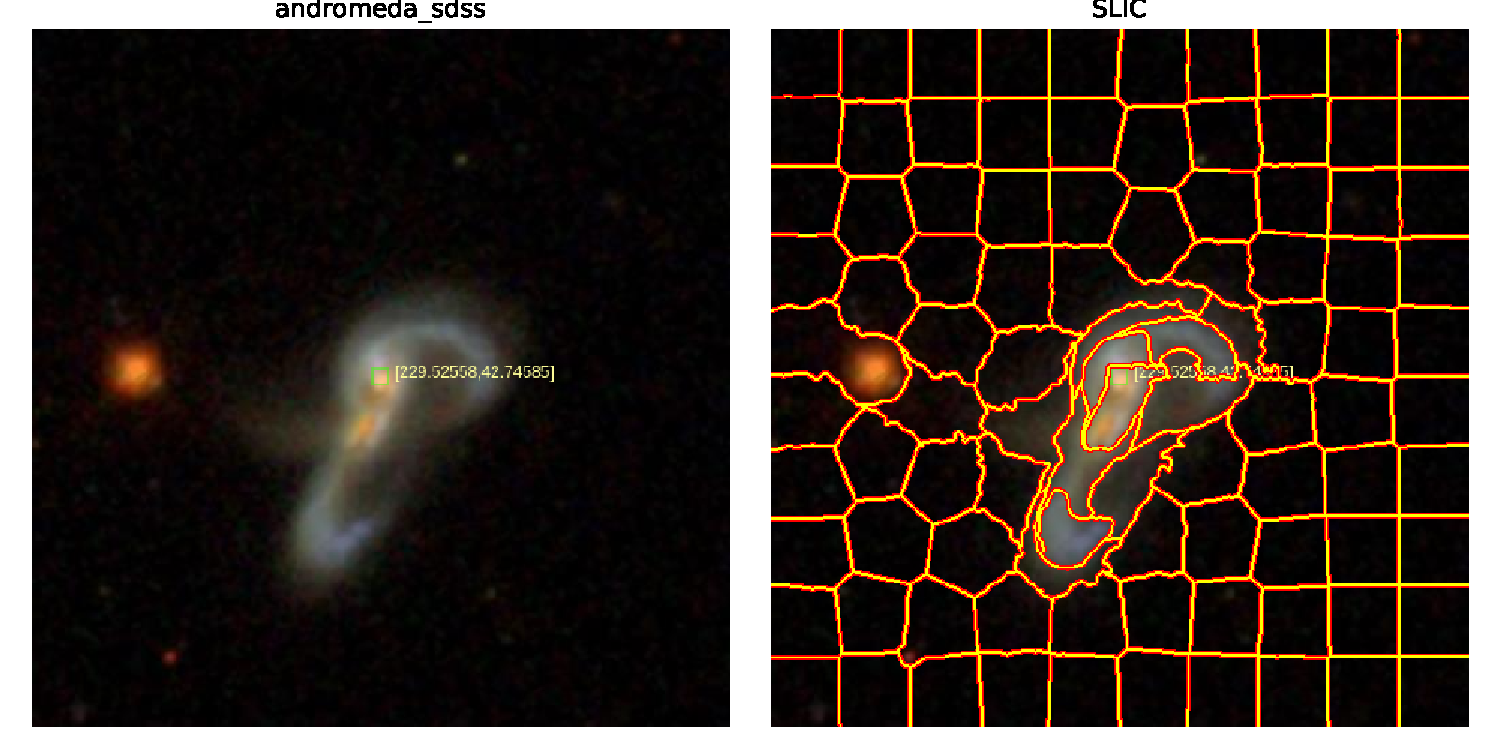
\includegraphics[width=0.99\textwidth]{../figures/segmented_andromeda_sdss.pdf}
    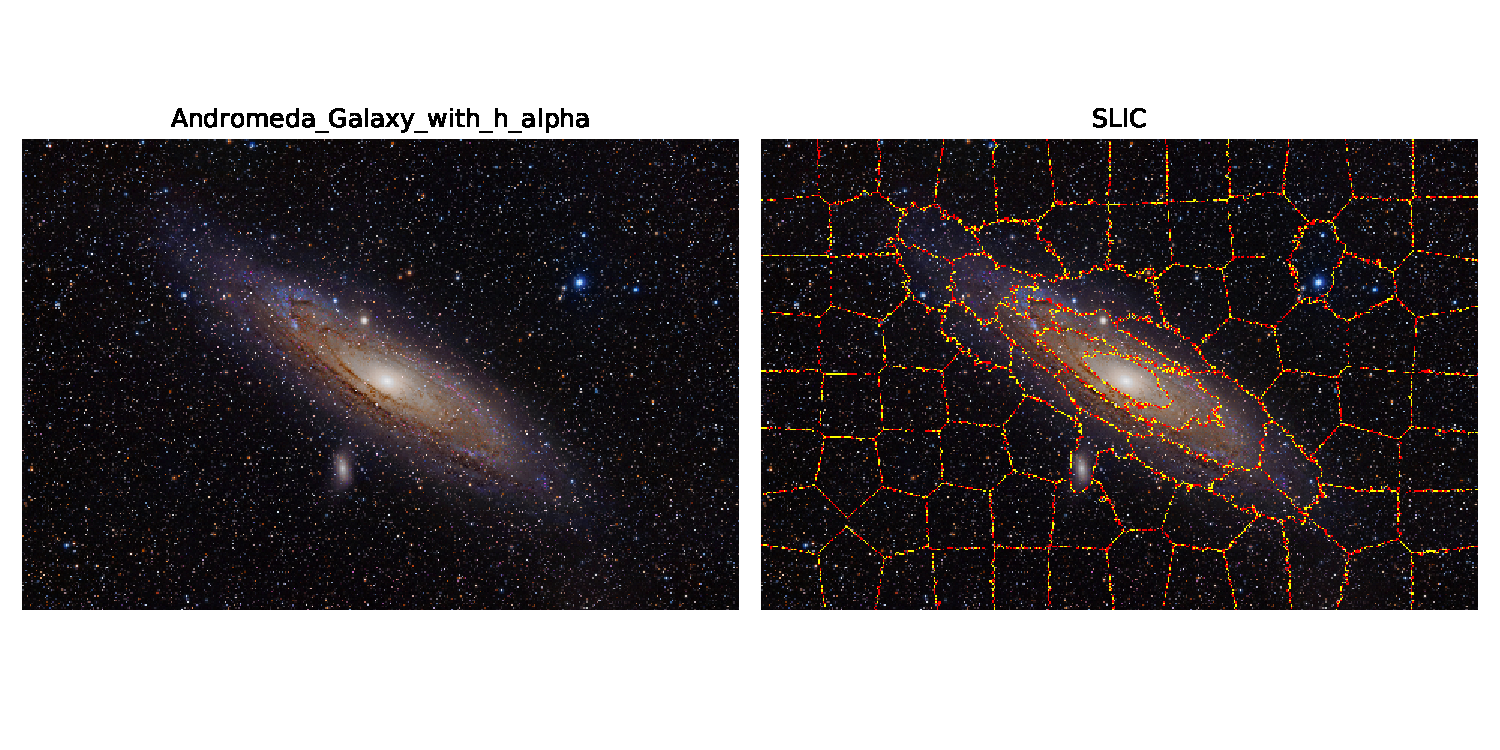
\includegraphics[width=0.99\textwidth]{../figures/segmented_Andromeda_Galaxy_with_h_alpha.pdf}

  \caption{\small{Two examples of segmented images for the Andromeda galaxy. Up: SDSS, Down: HST (review) }}
  \label{fig: andromeda segmented}
\end{figure}


To address the desireata exposed above, \cite{ribeiro2016}...
